% Biên dịch riêng mục 3.3 để xem trước (XeLaTeX):
%   cd report/query
%   latexmk -xelatex bao-cao-3.3.tex
% Nội dung nằm ở noi-dung.tex; báo cáo chung chỉ cần \input{query/noi-dung} và thêm query/query.bib.
\documentclass[12pt,a4paper]{article}

\usepackage{fontspec}
\setmainfont{Times New Roman}
\IfFontExistsTF{Consolas}{\setmonofont{Consolas}[Scale=0.9]}{\setmonofont{Courier New}}
\usepackage[margin=2.5cm]{geometry}
\usepackage{graphicx}
\usepackage{booktabs}
\usepackage{tabularx}
\usepackage{array}
\usepackage{float}
\usepackage[font=small,labelfont=bf]{caption}
\usepackage{fvextra}
\fvset{breaklines=true}
\usepackage{enumitem}
\usepackage{pgfplots}
\pgfplotsset{compat=1.18}
\usepackage{xcolor}
\usepackage[hidelinks]{hyperref}

\graphicspath{{images/}}
\renewcommand{\figurename}{Hình}
\renewcommand{\tablename}{Bảng}
\renewcommand{\refname}{Tài liệu tham khảo}
\setcounter{secnumdepth}{3}
\setlength{\emergencystretch}{2em}

\begin{document}

\setcounter{section}{2}
\section{So sánh Oracle và Redis}
\setcounter{subsection}{2}
% 3.3 Query processing. Người viết: Nguyễn Công Thành (TV3).
% File này chỉ chứa nội dung, được \input vào báo cáo chung (xem bao-cao-3.3.tex để biên dịch riêng).
% Báo cáo chung cần: fontspec (XeLaTeX), graphicx, booktabs, tabularx, fvextra, pgfplots, float, caption, hyperref,
% \graphicspath chứa thư mục query/images/ và file query/query.bib trong danh sách bibliography.
% Nhãn đều có tiền tố "q-" để không trùng với phần của người khác.

\subsection{Query processing}\label{sec:q}

\noindent\textit{Người viết: Nguyễn Công Thành}

Phần này so sánh cách Oracle và Redis xử lý cùng một truy vấn báo cáo, qua hai chức năng của ShopFlash: F5 (báo cáo doanh thu theo tháng, theo danh mục) và F6 (top sản phẩm bán chạy, khách VIP, sản phẩm chưa từng bán). Mỗi báo cáo được cài trên cả hai DBMS và trả cùng một kết quả, nên khác biệt đo được chỉ đến từ cách DBMS xử lý truy vấn.

\subsubsection*{Môi trường đo}

\begin{table}[H]
\centering
\caption{Môi trường đo của phần Query processing}\label{tab:q-env}
\small
\begin{tabularx}{\linewidth}{@{}lX@{}}
\toprule
Thành phần & Giá trị \\
\midrule
Máy & AMD Ryzen 5 7535HS, 15,3 GB RAM, SSD NVMe \\
Hệ điều hành, Docker & Windows 11 (10.0.26300), Docker 29.5.2 (cấp 12 CPU, 7,8 GB RAM) \\
Oracle & Oracle AI Database 26ai Free 23.26.3, image \texttt{database/free@sha256:f988b0c0\ldots8fba}. Oracle Free giới hạn 2 CPU, 2 GB RAM, 12 GB dữ liệu \\
Redis & Redis Stack 7.4.7 (RediSearch, RedisJSON), image \texttt{redis-stack-server@sha256:798ab84d\ldots742a} \\
Dữ liệu & 100.000 đơn, trong đó 87.141 đơn được tính (CONFIRMED, COMPLETED) với 215.807 dòng hàng; 10.001 sản phẩm, 51 danh mục, 20.002 người dùng. Redis: 87.141 document đơn, 215.807 document dòng hàng \\
\bottomrule
\end{tabularx}
\end{table}

Mỗi phép đo: chạy khởi động 1 lần không tính, sau đó đo 5 lần liên tiếp (không chạy song song), báo cáo trung bình $\pm$ độ lệch chuẩn, kèm p50 và p95. Thời gian đo trong backend, quanh lời gọi tới DB (gồm mạng tới container và đọc kết quả, không gồm HTTP tới trình duyệt). Khoảng thời gian của mọi báo cáo: 12 tháng gần nhất (01/11/2025 đến 18/10/2026). Số liệu thô nằm trong \texttt{report/query/results/}, cách chạy lại ở \texttt{report/query/README.md}, toàn bộ câu SQL và lệnh Redis ở Phụ lục C.

Hai trang của ứng dụng dùng trong phần này là trang \textit{Báo cáo} (Hình~\ref{fig:q-reports}) và trang \textit{So sánh Oracle--Redis}, nơi mỗi tab ứng với một demo dưới đây.

\begin{figure}[H]
\centering
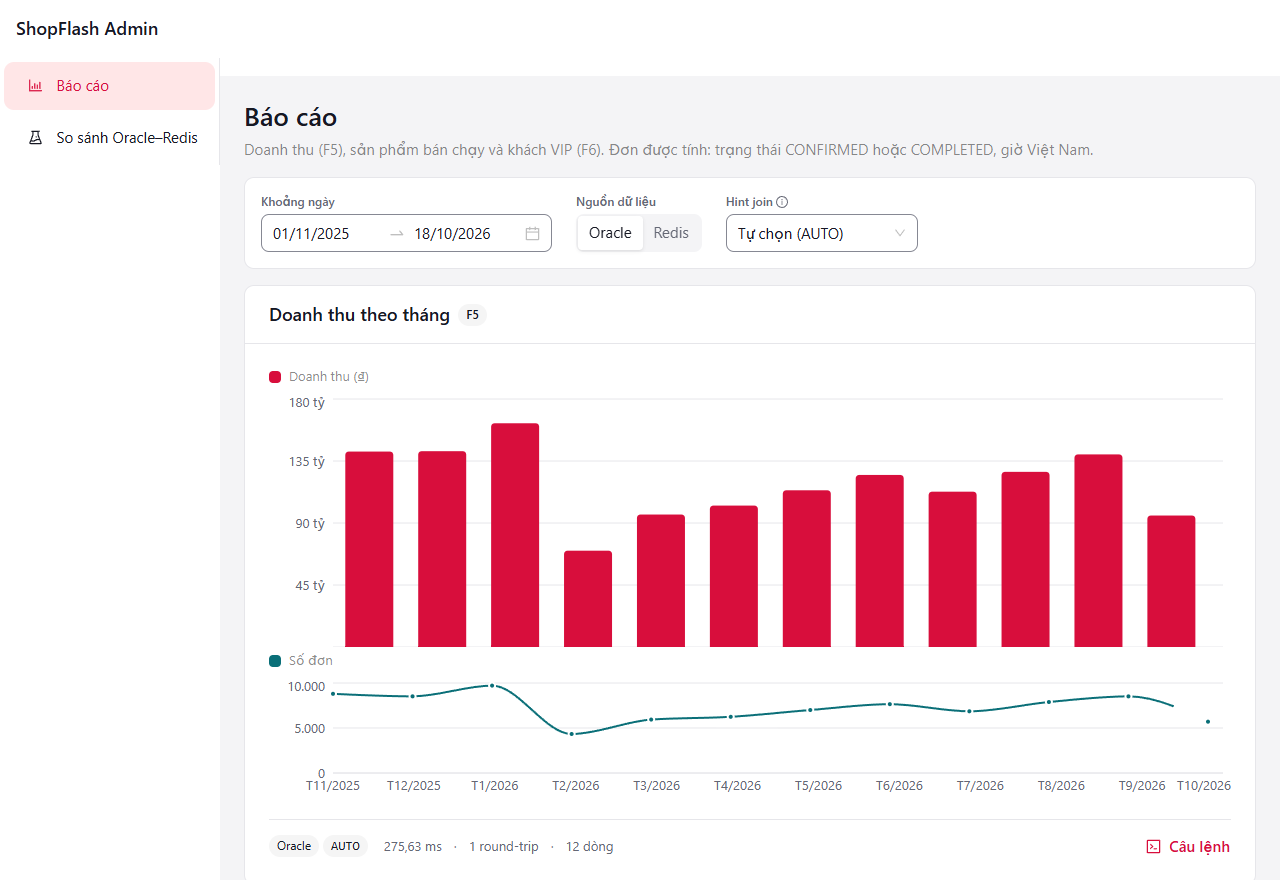
\includegraphics[width=0.85\linewidth]{3.3-01a-bao-cao-oracle-dau-trang.png}
\caption{Trang Báo cáo (F5, F6), nguồn Oracle. Mỗi khối báo cáo ghi nguồn, kiểu join, thời gian, số round-trip, số dòng và có nút xem câu lệnh}\label{fig:q-reports}
\end{figure}

% ---------------------------------------------------------------------------------------------
\subsubsection{Lý thuyết}\label{sec:q-theory}

Xử lý truy vấn là quá trình DBMS biến một câu truy vấn khai báo (``muốn gì'') thành một chuỗi thao tác cụ thể (``làm thế nào'') rồi thực thi nó. Theo \cite{q-silberschatz}, quá trình gồm ba bước:
\begin{enumerate}
  \item \textbf{Phân tích và dịch:} kiểm tra cú pháp, ngữ nghĩa, dịch câu SQL sang biểu thức đại số quan hệ.
  \item \textbf{Tối ưu:} sinh nhiều kế hoạch thực thi tương đương và chọn kế hoạch có chi phí ước lượng thấp nhất.
  \item \textbf{Thực thi:} chạy kế hoạch đã chọn, trả kết quả.
\end{enumerate}

Các khái niệm dùng trong phần này:
\begin{itemize}
  \item \textbf{Kế hoạch thực thi (execution plan):} cây các toán tử (quét bảng, quét index, join, gom nhóm, sắp xếp). Cùng một câu SQL có thể có nhiều kế hoạch cho cùng kết quả nhưng chi phí rất khác nhau.
  \item \textbf{Ba thuật toán join:}
  \begin{itemize}
    \item \textit{Nested loops:} với mỗi dòng của bảng ngoài, tìm các dòng khớp ở bảng trong (thường qua index). Tốt khi bảng ngoài ít dòng.
    \item \textit{Hash join:} dựng bảng băm trên bảng nhỏ hơn rồi quét bảng kia một lần. Tốt khi cả hai bảng lớn và điều kiện là phép bằng.
    \item \textit{Sort-merge join:} sắp hai bảng theo khóa join rồi trộn. Tốt khi dữ liệu đã có thứ tự sẵn.
  \end{itemize}
  \item \textbf{Tối ưu dựa trên chi phí (cost-based optimization):} chi phí của một kế hoạch được ước lượng từ \textbf{thống kê} (số dòng, số giá trị khác nhau, phân bố dữ liệu). Ước lượng số dòng (cardinality) sai thì có thể chọn sai kế hoạch.
  \item \textbf{Biến đổi truy vấn:} trước khi chọn kế hoạch, bộ tối ưu có thể viết lại truy vấn: gom nhóm sớm trước khi join, biến subquery \texttt{NOT EXISTS} thành anti-join, chỉ tính subquery không phụ thuộc một lần.
  \item \textbf{Pipeline cố định, không có bộ tối ưu:} một số hệ thống (như Redis) chỉ thực thi các bước đúng theo thứ tự người viết lệnh, không tự chọn hay đổi kế hoạch.
\end{itemize}

% ---------------------------------------------------------------------------------------------
\subsubsection{Trên Oracle}\label{sec:q-oracle}

Oracle có bộ tối ưu dựa trên chi phí (CBO) \cite{q-oracle-optimizer}. Với mỗi câu SQL, CBO dùng thống kê trong data dictionary để ước lượng số dòng ở từng bước, thử các thứ tự join, thuật toán join và cách truy cập (quét bảng hay index), rồi chọn kế hoạch rẻ nhất. Kế hoạch được lưu trong shared pool để dùng lại cho các lần chạy sau.

Cách xem kế hoạch trong phần này: thêm hint \texttt{GATHER\_PLAN\_STATISTICS} vào câu SQL, chạy, rồi gọi \texttt{DBMS\_XPLAN.DISPLAY\_CURSOR(NULL, NULL, 'ALLSTATS LAST')} trên cùng session \cite{q-oracle-xplan}. Cách này cho cả số dòng ước lượng (\texttt{E-Rows}) lẫn số dòng thực tế (\texttt{A-Rows}), thời gian thực tế (\texttt{A-Time}) và số block đọc (\texttt{Buffers}) của từng bước.

\paragraph{Demo 1: Kế hoạch CBO tự chọn cho báo cáo join 4 bảng}\label{sec:q-demo1}
\begin{description}
  \item[Mục đích:] cho thấy CBO tự chọn thuật toán join và tự viết lại truy vấn để giảm khối lượng công việc.
  \item[Cách làm:] chạy báo cáo top sản phẩm (F6). Câu SQL join \texttt{orders}, \texttt{order\_items}, \texttt{products}, \texttt{categories}, gom nhóm theo sản phẩm, lấy 10 sản phẩm bán nhiều nhất. Không thêm hint nào.
  \item[Kết quả:] kế hoạch \texttt{2314863829}, $155{,}2 \pm 23{,}6$ ms, đọc 5.104 block.
\end{description}
\begin{Verbatim}[fontsize=\scriptsize,frame=single]
| Id | Operation                  | Name        | E-Rows | A-Rows | Buffers |
|  4 |     HASH JOIN              |             |   9004 |   9001 |    5104 |
|  5 |      TABLE ACCESS FULL     | CATEGORIES  |     51 |     51 |       6 |
|  6 |      HASH JOIN             |             |   9004 |   9001 |    5098 |
|  7 |       VIEW                 | VW_GBC_17   |   9001 |   9001 |    4851 |
|  8 |        HASH GROUP BY       |             |   9001 |   9001 |    4851 |
| 10 |          HASH JOIN         |             |    213K|    215K|    4851 |
| 11 |           TABLE ACCESS FULL| ORDERS      |  87141 |  87141 |    2139 |
| 12 |           TABLE ACCESS FULL| ORDER_ITEMS |    247K|    247K|    2712 |
| 13 |       TABLE ACCESS FULL    | PRODUCTS    |  10001 |  10001 |     247 |
\end{Verbatim}
\begin{description}
  \item[Nhận xét:]\leavevmode
  \begin{itemize}
    \item CBO chọn \textbf{hash join} cho cả ba phép join và quét toàn bảng, vì báo cáo cần gần hết dữ liệu (87.141 trên 100.000 đơn). Dùng index để lấy từng dòng khi đó sẽ đắt hơn.
    \item CBO đã \textbf{viết lại truy vấn}. View \texttt{VW\_GBC\_17} là phép biến đổi \textit{group-by placement}: gom 215 nghìn dòng hàng theo sản phẩm \emph{trước} (còn 9.001 dòng), rồi mới join với \texttt{products} và \texttt{categories}. Câu SQL gốc viết join trước rồi mới \texttt{GROUP BY}.
    \item Số dòng ước lượng gần đúng tuyệt đối (9.004 so với 9.001), nhờ thống kê đã thu thập.
  \end{itemize}
\end{description}

\paragraph{Demo 2: Ép phương pháp join bằng hint}\label{sec:q-demo2}
\begin{description}
  \item[Mục đích:] chứng minh lựa chọn của CBO là đúng, bằng cách ép các thuật toán join khác và đo.
  \item[Cách làm:] chạy lại báo cáo doanh thu theo danh mục, top sản phẩm và khách VIP với 4 biến thể: AUTO (không hint) và 3 hint \texttt{LEADING(o oi p c) USE\_NL(oi p c)}, \texttt{USE\_HASH}, \texttt{USE\_MERGE}. \texttt{LEADING} giữ cố định thứ tự join, để hint thuật toán áp lên đúng từng bảng.
  \item[Kết quả:] Bảng~\ref{tab:q-hints} và Hình~\ref{fig:q-optimizer}.
\end{description}

\begin{table}[H]
\centering
\caption{Thời gian (ms) khi ép phương pháp join, trung bình $\pm$ độ lệch chuẩn của 5 lần đo}\label{tab:q-hints}
\small
\begin{tabular}{@{}lrrrr@{}}
\toprule
Báo cáo & AUTO & NL & HASH & MERGE \\
\midrule
Doanh thu theo danh mục & \textbf{208,5 $\pm$ 40,7} & 1.180,9 $\pm$ 227,9 & 233,2 $\pm$ 50,6 & 411,9 $\pm$ 82,4 \\
Top sản phẩm & \textbf{155,2 $\pm$ 23,6} & 852,9 $\pm$ 117,1 & 233,5 $\pm$ 28,6 & 573,5 $\pm$ 87,7 \\
Khách VIP (join 2 bảng) & 193,7 $\pm$ 24,4 & 271,7 $\pm$ 16,9 & \textbf{187,2 $\pm$ 6,8} & 250,6 $\pm$ 36,9 \\
\bottomrule
\end{tabular}
\end{table}

Kế hoạch NL của top sản phẩm (\texttt{2442890914}) đọc \textbf{681 nghìn block}, gấp 133 lần kế hoạch AUTO (5.104 block):
\begin{Verbatim}[fontsize=\scriptsize,frame=single]
| Id | Operation                          | Name                 | Starts | A-Rows | Buffers |
| 10 |           TABLE ACCESS FULL        | ORDERS               |      1 |  87141 |    2139 |
| 12 |            INDEX RANGE SCAN        | IX_ORDER_ITEMS_ORDER |  87141 |    215K|   26868 |
| 14 |           INDEX UNIQUE SCAN        | PK_PRODUCTS          |    215K|    215K|    215K |
| 16 |        TABLE ACCESS BY INDEX ROWID | CATEGORIES           |    215K|    215K|    215K |
\end{Verbatim}

\begin{figure}[H]
\centering
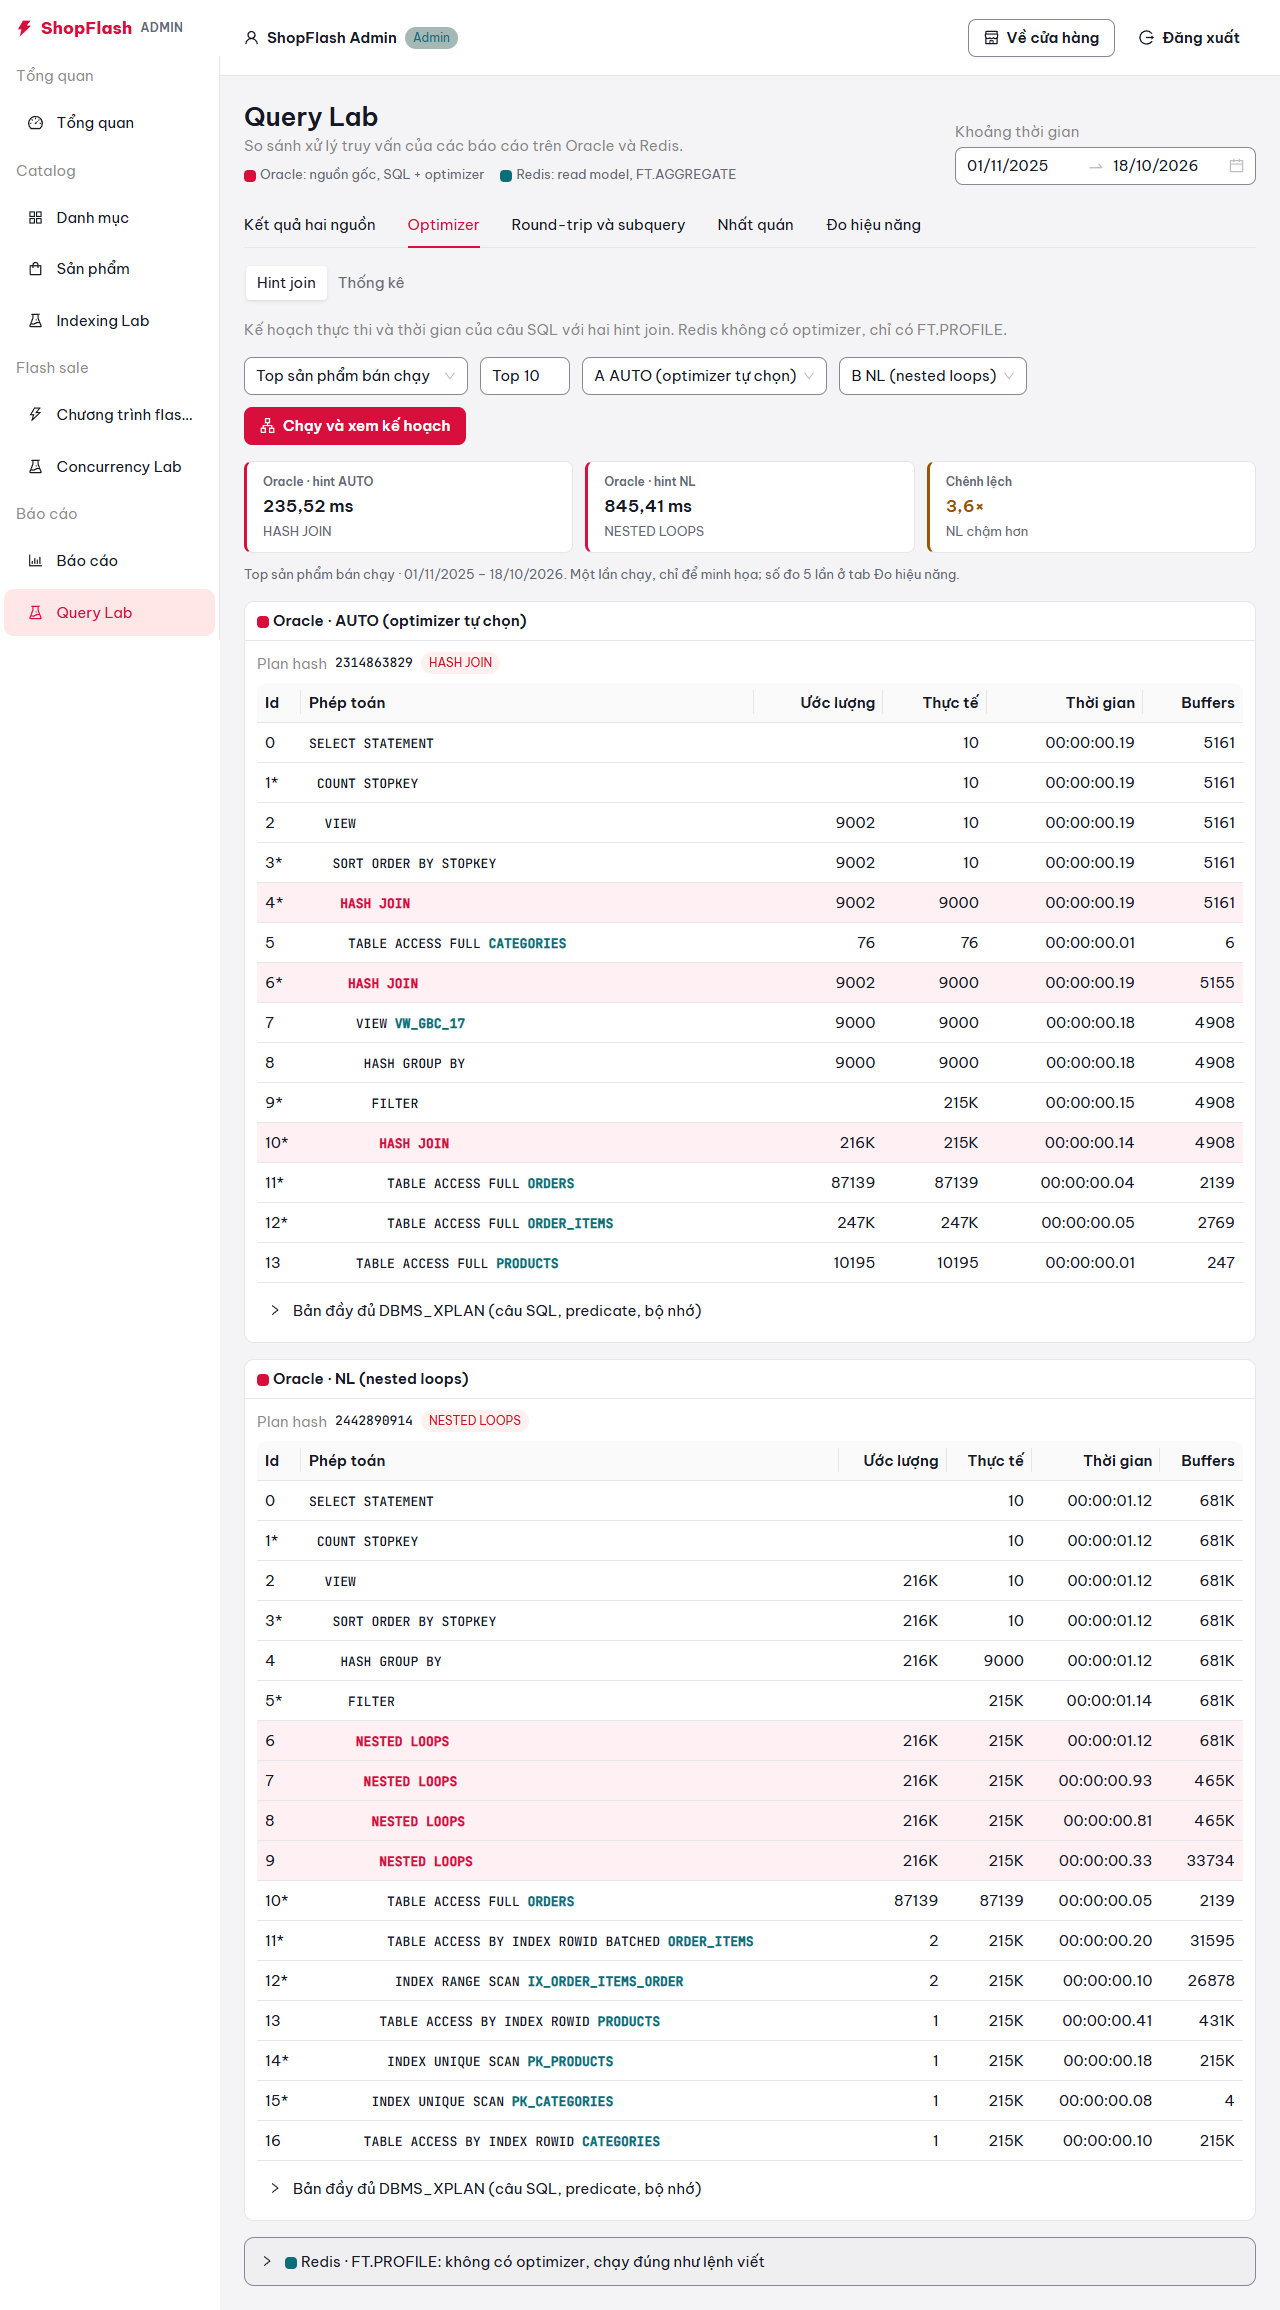
\includegraphics[width=0.8\linewidth]{3.3-04-d2-optimizer.png}
\caption{Tab Optimizer: cùng câu SQL top sản phẩm, trái là kế hoạch CBO tự chọn (HASH JOIN), phải là kế hoạch bị ép NESTED LOOPS; bên dưới là \texttt{FT.PROFILE} của Redis cho cùng báo cáo}\label{fig:q-optimizer}
\end{figure}

\begin{description}
  \item[Nhận xét:]\leavevmode
  \begin{itemize}
    \item Ép nested loops làm hai báo cáo join 4 bảng chậm đi 5,5--5,7 lần. Cột \texttt{Starts} cho thấy lý do: index của \texttt{order\_items} được dò 87.141 lần, index của \texttt{products} và \texttt{categories} mỗi cái 215 nghìn lần, mỗi lần đọc ít nhất một block.
    \item Kế hoạch AUTO nhanh nhất hoặc ngang với kế hoạch tốt nhất ở mọi báo cáo. Ở báo cáo khách VIP, HASH nhanh hơn AUTO 6,5 ms nhưng nằm trong độ lệch chuẩn, vì AUTO cũng chọn hash join. Lập trình viên chỉ viết câu SQL, CBO tự chọn được cách chạy tốt.
  \end{itemize}
\end{description}

\paragraph{Demo 3: Thống kê quyết định kế hoạch}\label{sec:q-demo3}
\begin{description}
  \item[Mục đích:] cho thấy CBO phụ thuộc vào thống kê: thống kê mất thì ước lượng sai, kế hoạch đổi và chậm hơn.
  \item[Cách làm:] với báo cáo top sản phẩm:
  \begin{enumerate}
    \item Lấy kế hoạch khi có thống kê.
    \item Gọi \texttt{DBMS\_STATS.DELETE\_TABLE\_STATS} cho 5 bảng rồi lấy lại kế hoạch.
    \item Gọi \texttt{DBMS\_STATS.GATHER\_TABLE\_STATS} rồi lấy lại kế hoạch.
  \end{enumerate}
  Cả hai thủ tục đều phải truyền \texttt{no\_invalidate => FALSE} \cite{q-oracle-stats}. Nếu để mặc định, Oracle dùng lại kế hoạch cũ đang lưu trong shared pool và không thấy thay đổi gì.
  \item[Kết quả:] Bảng~\ref{tab:q-stats}. Hình~\ref{fig:q-stats} là tab Thống kê ở trạng thái ban đầu, trước khi xóa.
\end{description}

\begin{table}[H]
\centering
\caption{Kế hoạch của báo cáo top sản phẩm theo trạng thái thống kê (số dòng thực tế sau gom nhóm: 9.001)}\label{tab:q-stats}
\small
\begin{tabular}{@{}llllrr@{}}
\toprule
Trạng thái & Plan hash & Phép join chính & Ước lượng sau gom nhóm & Buffers & A-Time \\
\midrule
Có thống kê & 2314863829 & HASH JOIN & 9.004 & 5.104 & 0,18 s \\
Đã xóa thống kê & \textbf{56634007} & \textbf{MERGE JOIN} & \textbf{285.000} & \textbf{90.978} & \textbf{0,58 s} \\
Thu thập lại & 2314863829 & HASH JOIN & 9.003 & 5.104 & 0,21 s \\
\bottomrule
\end{tabular}
\end{table}

Trích kế hoạch khi đã xóa thống kê:
\begin{Verbatim}[fontsize=\scriptsize,frame=single]
| Id | Operation                              | Name                     | Starts | E-Rows | A-Rows | Buffers |
|  5 |      MERGE JOIN                        |                          |      1 |    285K|   9001 |   90978 |
| 12 |             TABLE ACCESS BY INDEX ROWID| ORDERS                   |      2 |  89730 |  87141 |   88010 |
| 13 |              INDEX RANGE SCAN          | IX_ORDERS_STATUS_CREATED |      2 |      2 |  87141 |     916 |
Note
   - dynamic statistics used: dynamic sampling (level=2)
\end{Verbatim}

\begin{figure}[H]
\centering
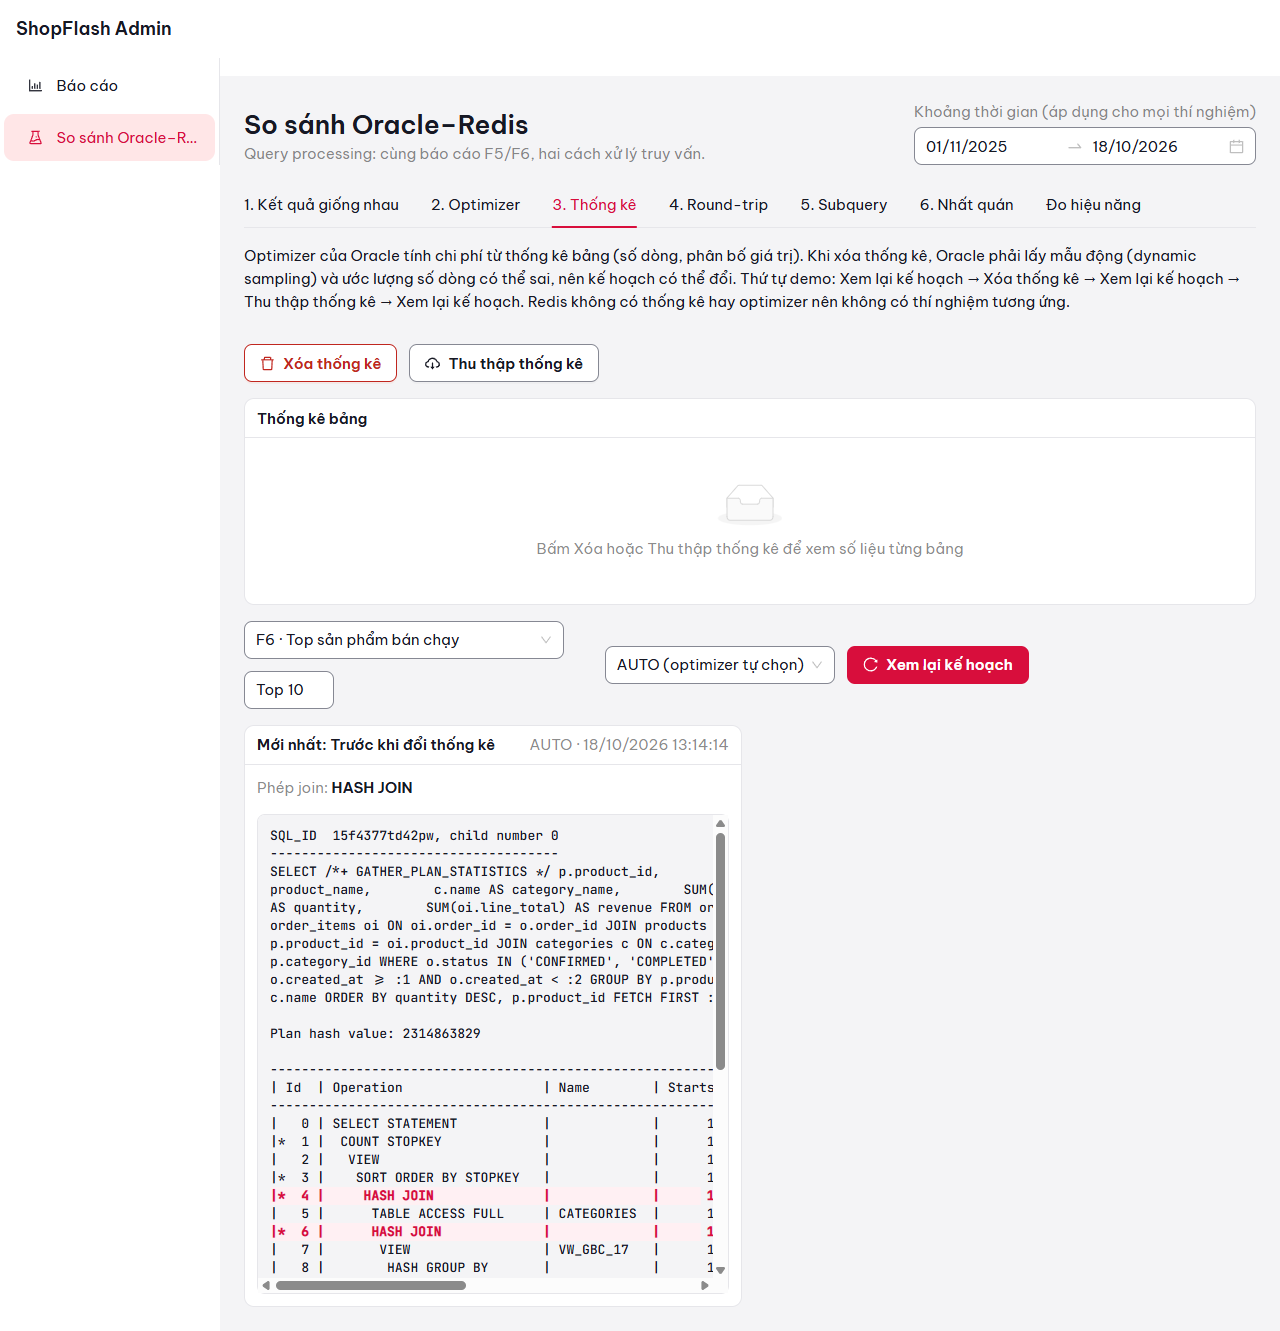
\includegraphics[width=0.75\linewidth]{3.3-05-d3-thong-ke.png}
\caption{Tab Thống kê: nút Xóa / Thu thập thống kê và kế hoạch hiện tại (đang là HASH JOIN, trước khi xóa thống kê)}\label{fig:q-stats}
\end{figure}

\begin{description}
  \item[Nhận xét:]\leavevmode
  \begin{itemize}
    \item Không có thống kê, Oracle phải lấy mẫu nhanh lúc parse (dynamic sampling). Ước lượng lệch nhiều: index \texttt{IX\_ORDERS\_STATUS\_CREATED} được ước lượng trả về 2 dòng, thực tế 87.141; kết quả gom nhóm được ước lượng 285 nghìn dòng, thực tế 9.001.
    \item Do tin rằng điều kiện lọc rất chọn lọc, CBO đi qua index rồi đọc từng dòng của \texttt{orders} (88.010 block, hơn 17 lần cả kế hoạch cũ) và chuyển sang merge join. Thời gian tăng hơn 3 lần.
    \item Thu thập lại thống kê thì kế hoạch quay về đúng như ban đầu. Kế hoạch tốt phụ thuộc vào thống kê đúng, nên trong vận hành cần để job thu thập thống kê tự động của Oracle chạy, đặc biệt sau khi nạp nhiều dữ liệu.
  \end{itemize}
\end{description}

\paragraph{Demo 4: Subquery được biến đổi thế nào}\label{sec:q-demo4}
\begin{description}
  \item[Mục đích:] cho thấy Oracle chạy được subquery ngay trong SQL và biến đổi nó thành phép toán hiệu quả.
  \item[Cách làm:] hai báo cáo F6. \textit{Khách VIP}: khách có tổng chi lớn hơn mức trung bình, dùng subquery trong \texttt{HAVING}. \textit{Sản phẩm chưa từng bán}: dùng \texttt{NOT EXISTS}.
\end{description}
\begin{Verbatim}[fontsize=\scriptsize,frame=single]
HAVING SUM(o.total_amount) > (
    SELECT AVG(t.spent)
    FROM (SELECT SUM(o2.total_amount) AS spent FROM orders o2
          WHERE o2.status IN ('CONFIRMED', 'COMPLETED') AND o2.created_at >= :fromTs
            AND o2.created_at < :toExclusiveTs
          GROUP BY o2.user_id) t)
...
WHERE p.status = 'ACTIVE'
  AND NOT EXISTS (SELECT 1 FROM order_items oi WHERE oi.product_id = p.product_id)
\end{Verbatim}
\begin{description}
  \item[Kết quả:] Bảng~\ref{tab:q-subquery}. Thời gian gồm 2 câu: câu lấy trang dữ liệu và câu tóm tắt (tổng số dòng, chi tiêu trung bình) để hiển thị và phân trang.
\end{description}

\begin{table}[H]
\centering
\caption{Subquery trên Oracle}\label{tab:q-subquery}
\small
\begin{tabularx}{\linewidth}{@{}lrX@{}}
\toprule
Báo cáo & Thời gian (ms) & Toán tử chính trong kế hoạch \\
\midrule
Khách VIP & 193,7 $\pm$ 24,4 & \texttt{FILTER} + \texttt{SORT AGGREGATE} chạy 1 lần (\texttt{Starts = 1}) \\
Sản phẩm chưa từng bán & 139,3 $\pm$ 22,8 & \texttt{HASH JOIN ANTI} + \texttt{INDEX FAST FULL SCAN} trên \texttt{IX\_ORDER\_ITEMS\_PRODUCT} \\
\bottomrule
\end{tabularx}
\end{table}

\begin{description}
  \item[Nhận xét:]\leavevmode
  \begin{itemize}
    \item Với khách VIP, subquery tính trung bình không phụ thuộc dòng ngoài, nên Oracle chỉ tính \textbf{một lần} rồi dùng để lọc 19.274 khách, còn lại 6.049 khách.
    \item Với sản phẩm chưa từng bán, Oracle biến \texttt{NOT EXISTS} thành \textbf{anti-join} dạng hash. Nó chỉ quét index trên \texttt{order\_items.product\_id} (không cần đọc bảng) để tìm 953 sản phẩm chưa xuất hiện trong dòng hàng nào.
    \item Người viết không cần biết các biến đổi này, CBO tự làm.
  \end{itemize}
\end{description}

% ---------------------------------------------------------------------------------------------
\subsubsection{Trên Redis}\label{sec:q-redis}

Redis là kho key-value, không có SQL, không có join và không có bộ tối ưu. Để làm báo cáo, ShopFlash dùng module \textbf{RediSearch} trên dữ liệu JSON (RedisJSON) \cite{q-redis-aggregations}:
\begin{itemize}
  \item \textbf{Read model đã denormalize.} Dữ liệu được dựng lại từ Oracle thành hai loại document:
  \begin{itemize}
    \item \texttt{order:analytics:\{orderId\}}: một đơn, đã kèm tên và email khách.
    \item \texttt{order:line:\{orderItemId\}}: một dòng hàng, đã kèm tên sản phẩm, mã và tên danh mục, trạng thái và ngày của đơn.
  \end{itemize}
  Join được làm sẵn một lần lúc dựng, không làm lúc truy vấn. Dựng lại 100.000 đơn mất khoảng 20--35 giây.
  \item \textbf{Index RediSearch} \texttt{idx:order-analytics} và \texttt{idx:order-line-analytics}: \texttt{status} là TAG, \texttt{createdAt} là NUMERIC, các trường dùng để gom nhóm, cộng dồn hoặc trả về khai báo \texttt{SORTABLE}.
  \item \textbf{\texttt{FT.AGGREGATE}} chạy một pipeline cố định: lọc theo index, rồi \texttt{GROUPBY}/\texttt{REDUCE}, \texttt{SORTBY}, \texttt{APPLY}/\texttt{FILTER}, \texttt{LIMIT}, đúng theo thứ tự các bước trong lệnh \cite{q-redis-commands}.
\end{itemize}

Để so sánh, mỗi báo cáo trên Redis được cài theo hai cách:
\begin{itemize}
  \item \textbf{AGGREGATE:} để Redis tự gom nhóm và sắp xếp, 1 lệnh.
  \item \textbf{CLIENT:} Redis chỉ lọc theo index và trả document thô theo từng trang (\texttt{WITHCURSOR}, 10.000 document mỗi trang). Ứng dụng Java tự gom nhóm và sắp xếp. Đây là cách làm khi coi Redis là kho key-value thuần.
\end{itemize}

\paragraph{Demo 5: Cùng kết quả trên hai nguồn}\label{sec:q-demo5}
\begin{description}
  \item[Mục đích:] đảm bảo các phép so sánh hiệu năng là công bằng: hai nguồn phải trả đúng cùng một kết quả.
  \item[Cách làm:] API \texttt{/compare} chạy một báo cáo trên Oracle và Redis rồi so từng dòng. Kiểm tra tự động bằng \texttt{tests/contract\_test.py} (146 kiểm tra) trên cả 4 báo cáo Redis hỗ trợ.
  \item[Kết quả:] cả 4 báo cáo khớp từng dòng, kể cả tổng tiền (VND). Hình~\ref{fig:q-match}.
  \item[Nhận xét:] kết quả khớp, nên mọi khác biệt về thời gian ở các demo sau đến từ cách xử lý truy vấn, không phải từ việc tính khác nhau.
\end{description}

\begin{figure}[H]
\centering
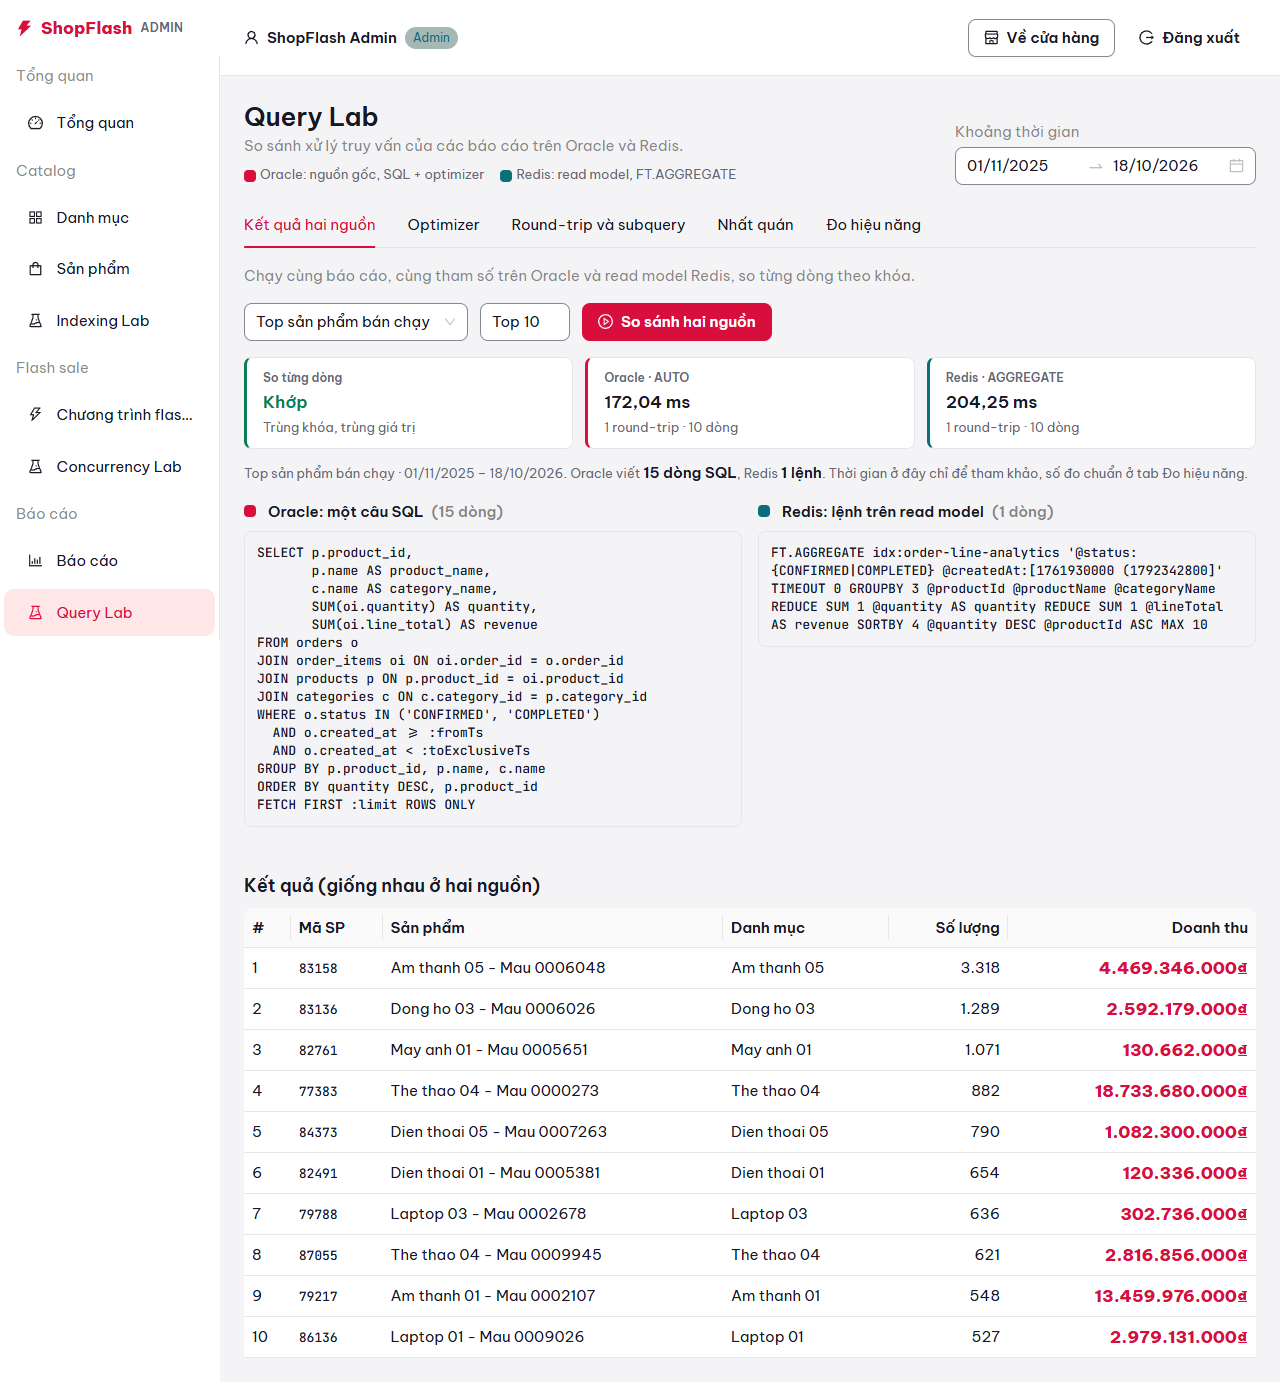
\includegraphics[width=0.75\linewidth]{3.3-03-d1-ket-qua-khop.png}
\caption{Tab Kết quả giống nhau: top 10 sản phẩm trên Oracle (trái) và Redis (phải) khớp từng dòng}\label{fig:q-match}
\end{figure}

\paragraph{Demo 6: Redis chạy đúng như lệnh viết}\label{sec:q-demo6}
\begin{description}
  \item[Mục đích:] cho thấy Redis không có bộ tối ưu: kế hoạch chính là thứ tự các bước người viết lệnh đặt ra.
  \item[Cách làm:] chạy \texttt{FT.PROFILE \ldots{} AGGREGATE} cho báo cáo doanh thu theo danh mục:
\end{description}
\begin{Verbatim}[fontsize=\scriptsize,frame=single]
FT.AGGREGATE idx:order-line-analytics
  '@status:{CONFIRMED|COMPLETED} @createdAt:[1761930000 (1792342800]' TIMEOUT 0
  GROUPBY 2 @categoryId @categoryName
  REDUCE SUM 1 @quantity AS quantity REDUCE SUM 1 @lineTotal AS revenue
  SORTBY 4 @revenue DESC @categoryId ASC
\end{Verbatim}
\begin{description}
  \item[Kết quả:] trích \texttt{results/plans/revenue-by-category-redis-AGGREGATE.txt}:
\end{description}
\begin{Verbatim}[fontsize=\scriptsize,frame=single]
Iterators profile:
  Type=INTERSECT, Counter=215807                     giao hai điều kiện lọc
    Type=UNION, Query type=TAG, Counter=215807       status: confirmed 61.781 + completed 154.026
    Type=UNION, Query type=NUMERIC, Counter=215807   createdAt: hợp nhiều khoảng số
Result processors profile:
  Type=Index,   Counter=215807
  Type=Grouper, Counter=51
  Type=Sorter,  Counter=51
\end{Verbatim}
\begin{description}
  \item[Nhận xét:]\leavevmode
  \begin{itemize}
    \item Kết quả profile chỉ là danh sách các bước theo đúng thứ tự trong lệnh: lọc theo index, gom nhóm, sắp xếp. Không có lựa chọn thuật toán hay biến đổi nào.
    \item Muốn chạy khác đi (ví dụ lọc thêm điều kiện trước khi gom), người viết phải tự viết lại lệnh.
    \item Mọi thứ CBO tự làm trong Demo 1 đều đã được lập trình viên làm trước: join lúc dựng read model, chọn trường \texttt{SORTABLE} lúc tạo index.
  \end{itemize}
\end{description}

\paragraph{Demo 7: Đẩy tính toán xuống Redis hay kéo về ứng dụng}\label{sec:q-demo7}
\begin{description}
  \item[Mục đích:] đo cái giá của việc kéo dữ liệu về ứng dụng để tính, so với để Redis tự tính.
  \item[Cách làm:] chạy 4 báo cáo theo hai cách AGGREGATE và CLIENT, đếm số round-trip tới Redis.
  \item[Kết quả:] Bảng~\ref{tab:q-roundtrip}. Hình~\ref{fig:q-roundtrip} là tab Round-trip của một lần chạy đơn lẻ (không phải số đo chính thức, máy đang chịu tải nên chênh lệch lớn hơn).
\end{description}

\begin{table}[H]
\centering
\caption{Redis: AGGREGATE so với CLIENT, thời gian (ms), 5 lần đo}\label{tab:q-roundtrip}
\small\setlength{\tabcolsep}{4pt}
\begin{tabular}{@{}lrrrr@{}}
\toprule
Báo cáo & AGGREGATE & CLIENT & Round-trip & CLIENT chậm hơn \\
\midrule
Doanh thu theo tháng & 199,9 $\pm$ 22,1 & 820,1 $\pm$ 55,2 & 9 & 4,1 lần \\
Doanh thu theo danh mục & 373,4 $\pm$ 48,5 & 2.597,1 $\pm$ 382,3 & 22 & 7,0 lần \\
Top sản phẩm & 850,7 $\pm$ 32,4 & 4.851,2 $\pm$ 1.463,0 & 22 & 5,7 lần \\
Khách VIP & 875,4 $\pm$ 76,8 & 2.362,9 $\pm$ 517,2 & 9 & 2,7 lần \\
\bottomrule
\end{tabular}
\end{table}

\begin{figure}[H]
\centering
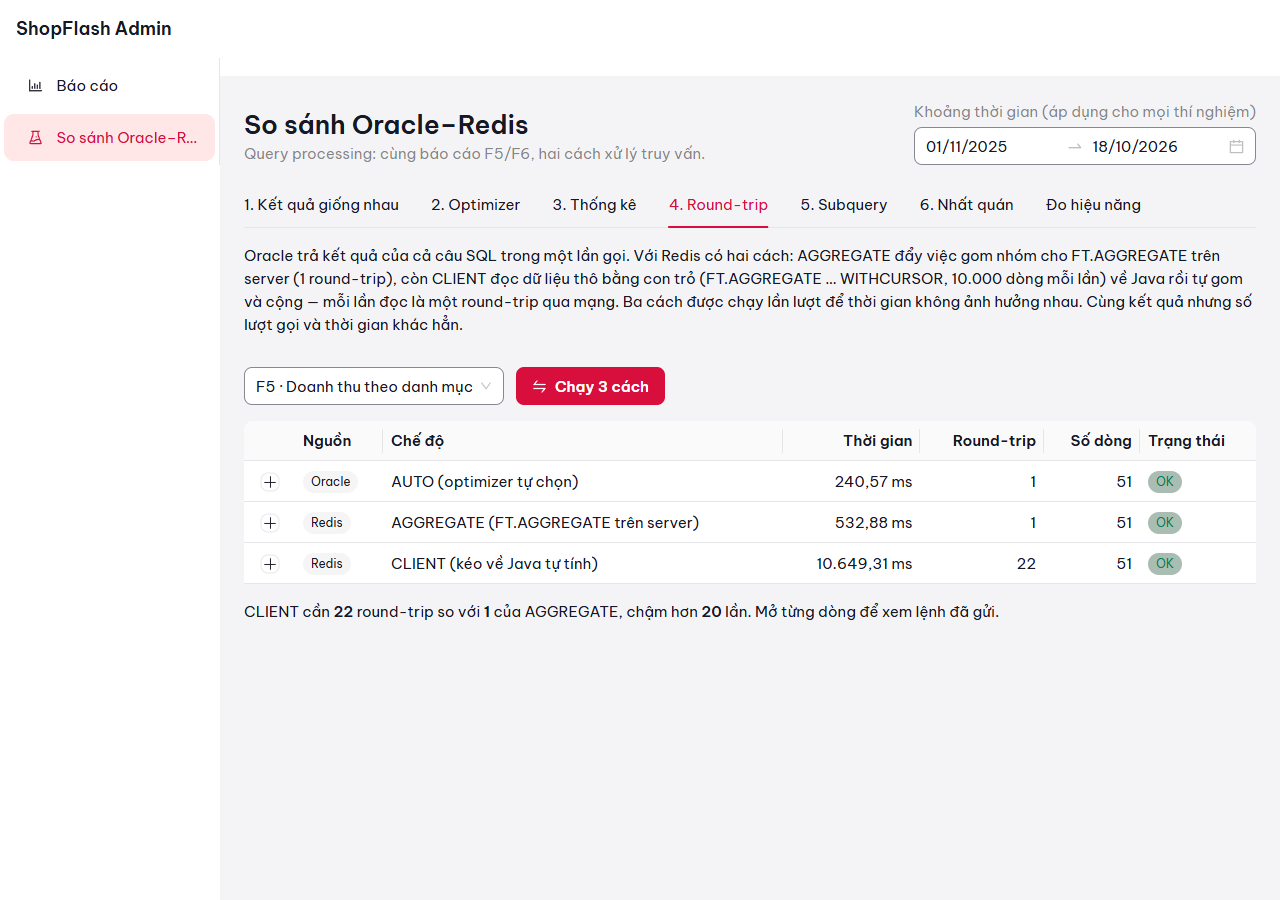
\includegraphics[width=0.75\linewidth]{3.3-06-d4-round-trip.png}
\caption{Tab Round-trip: cùng báo cáo doanh thu theo danh mục, Redis AGGREGATE cần 1 round-trip, CLIENT cần 22 (một lần chạy)}\label{fig:q-roundtrip}
\end{figure}

\begin{description}
  \item[Nhận xét:]\leavevmode
  \begin{itemize}
    \item Theo cách CLIENT, toàn bộ 215.807 dòng hàng (hoặc 87.141 đơn) phải đi qua mạng về ứng dụng, qua 9--22 lần gọi, chỉ để ra 51 dòng kết quả.
    \item Để Redis gom nhóm ngay tại chỗ chứa dữ liệu thì chỉ cần 1 lần gọi và trả về đúng số dòng cần.
    \item Báo cáo có ít nhóm (theo danh mục, 51 nhóm) được lợi nhiều nhất. Độ lệch chuẩn của CLIENT cũng lớn hơn hẳn, vì thời gian phụ thuộc vào mạng và bộ nhớ của ứng dụng.
  \end{itemize}
\end{description}

\paragraph{Demo 8: Không có subquery}\label{sec:q-demo8}
\begin{description}
  \item[Mục đích:] cho thấy giới hạn về khả năng biểu đạt của Redis so với SQL.
  \item[Cách làm:]\leavevmode
  \begin{itemize}
    \item \textit{Khách VIP:} \texttt{FT.AGGREGATE} không có subquery, nên phải chạy 2 lượt. Lượt 1 tính trung bình tổng chi mỗi khách. Lượt 2 gom nhóm theo khách rồi lọc bằng \texttt{FILTER} với điều kiện \texttt{@totalSpent > <trung bình>}, giá trị trung bình do ứng dụng chèn vào lệnh.
    \item \textit{Sản phẩm chưa từng bán:} cần anti-join.
  \end{itemize}
  \item[Kết quả:]\leavevmode
  \begin{itemize}
    \item Khách VIP: $875{,}4 \pm 76{,}8$ ms cho 2 lượt (Oracle: $193{,}7 \pm 24{,}4$ ms). Hình~\ref{fig:q-subquery}.
    \item Sản phẩm chưa từng bán: \textbf{không làm được}, API trả \texttt{meta.supported = false} (Hình~\ref{fig:q-unsupported}).
  \end{itemize}
\end{description}

\begin{figure}[H]
\centering
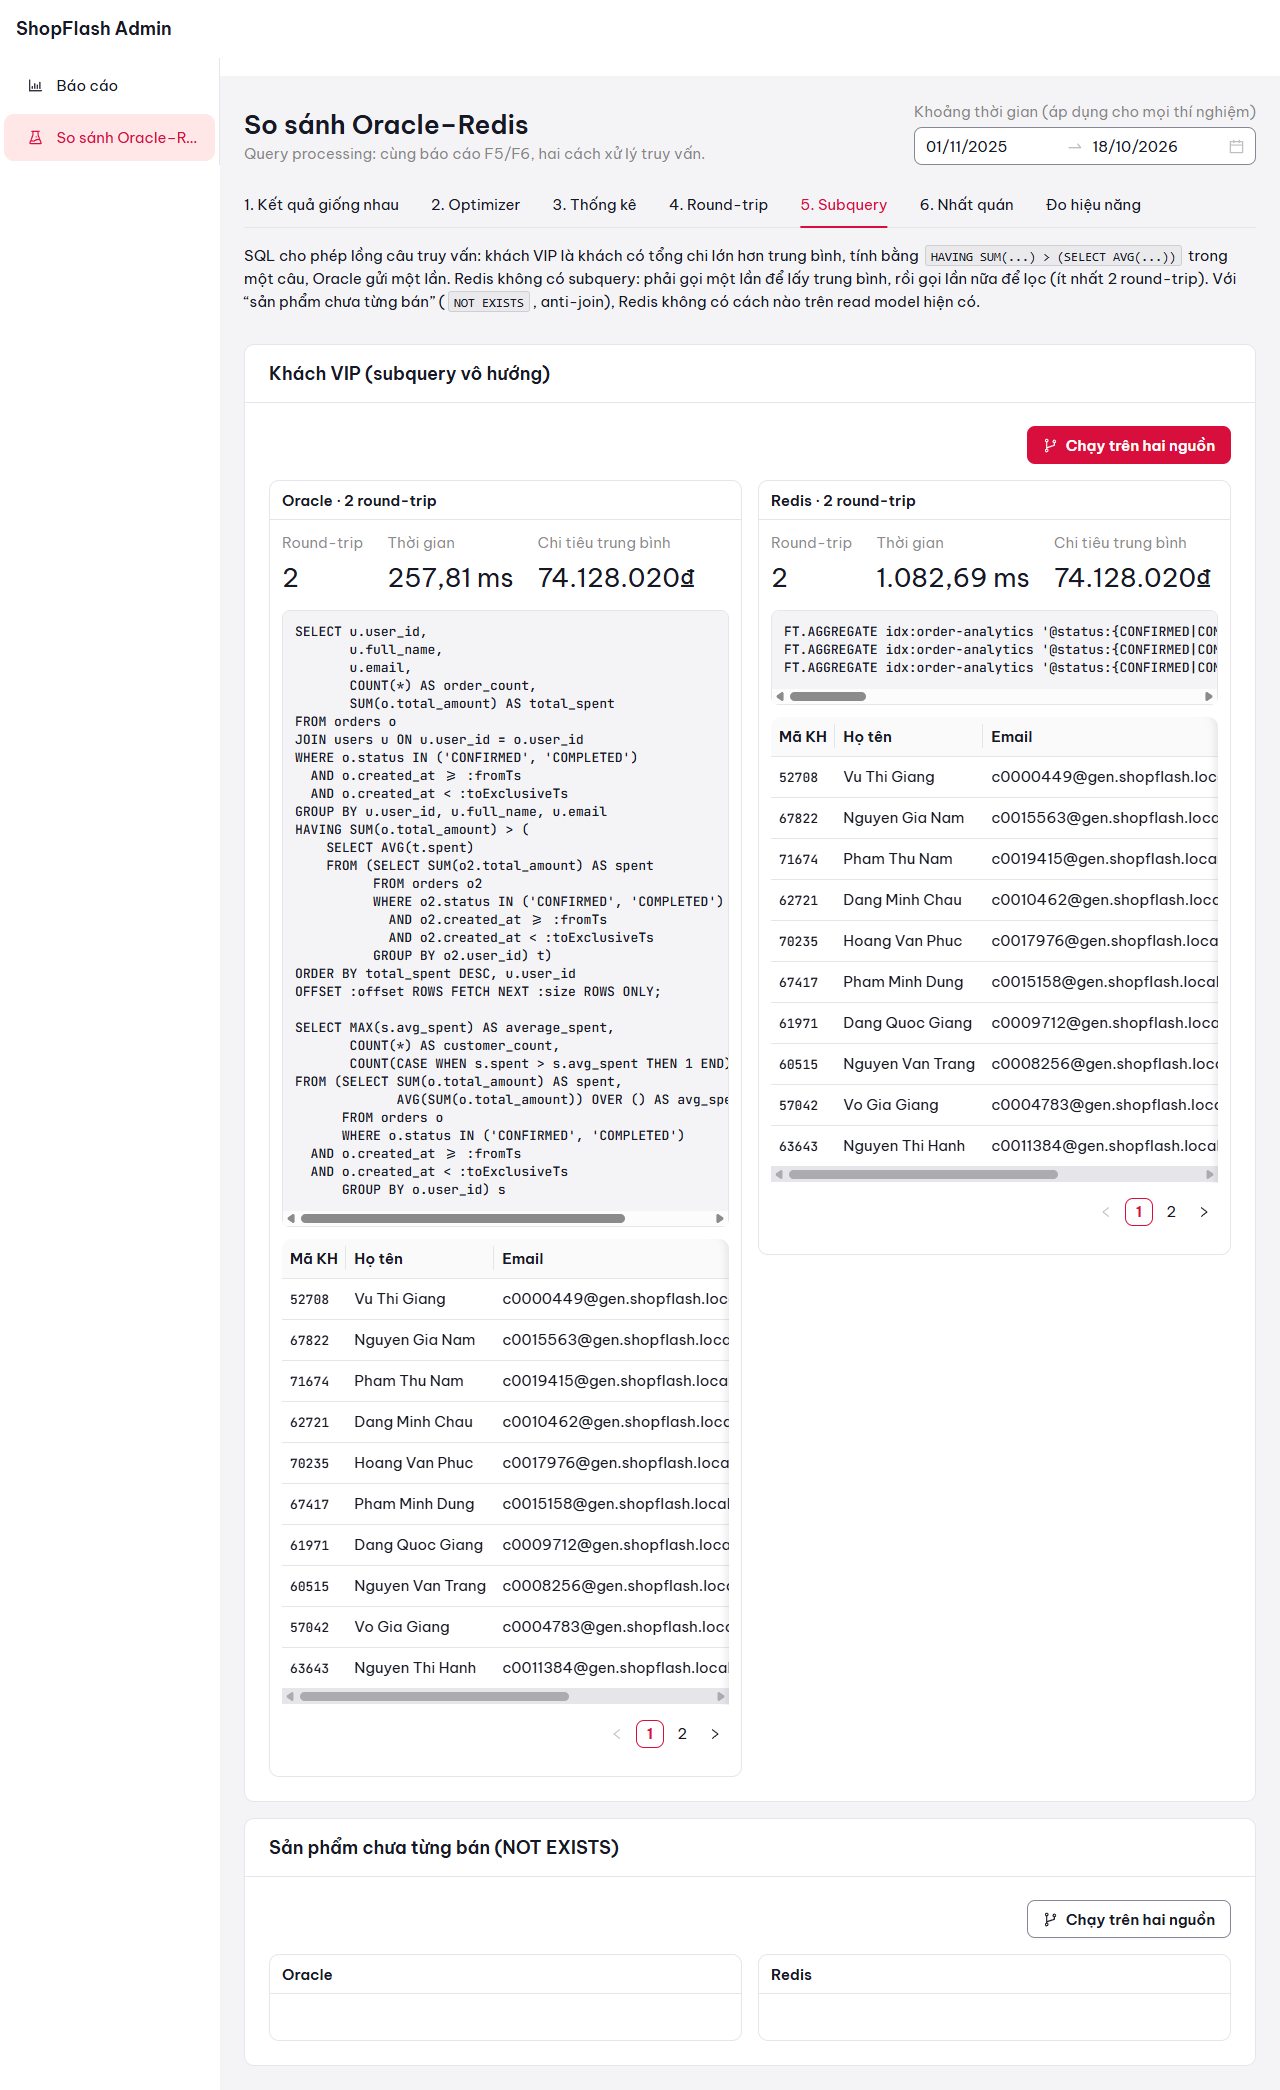
\includegraphics[width=0.7\linewidth]{3.3-07-d5-subquery.png}
\caption{Tab Subquery: khách VIP trên Oracle (1 câu SQL có subquery, kèm câu tóm tắt) và Redis (\texttt{FT.AGGREGATE} chạy 2 lượt), cùng chi tiêu trung bình 74.128.020\,₫}\label{fig:q-subquery}
\end{figure}

\begin{figure}[H]
\centering
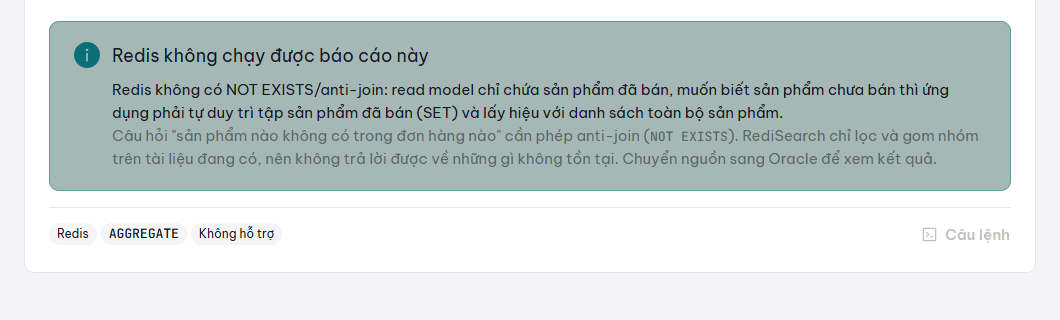
\includegraphics[width=0.8\linewidth]{3.3-02b-redis-chua-ban-khong-ho-tro.png}
\caption{Trang Báo cáo với nguồn Redis: báo cáo ``Sản phẩm chưa từng bán'' không chạy được}\label{fig:q-unsupported}
\end{figure}

\begin{description}
  \item[Nhận xét:]\leavevmode
  \begin{itemize}
    \item Ứng dụng phải tự tách truy vấn lồng nhau thành nhiều bước. Giữa hai lượt, dữ liệu có thể thay đổi, nên hai lượt có thể không nhìn cùng một trạng thái.
    \item ``Sản phẩm chưa từng bán'' cần so tập sản phẩm với tập dòng hàng. Read model chỉ chứa dòng hàng đã bán, Redis không có phép anti-join. Muốn làm phải dựng thêm một read model khác cho đúng câu hỏi này.
  \end{itemize}
\end{description}

\paragraph{Demo 9: Read model không tự cập nhật}\label{sec:q-demo9}
\begin{description}
  \item[Mục đích:] cho thấy cái giá của việc tách bản đọc riêng: dữ liệu báo cáo trên Redis bị trễ so với Oracle.
  \item[Cách làm:] kịch bản nằm trong \texttt{tests/contract\_test.py} (phần D6):
  \begin{enumerate}
    \item Chèn 1 đơn mới vào Oracle bằng SQL.
    \item Gọi \texttt{GET /analytics/status} và \texttt{/revenue-by-month/compare}.
    \item Dựng lại read model.
    \item So lại.
  \end{enumerate}
  \item[Kết quả:] sau khi chèn, \texttt{inSync = false} và compare báo lệch ở tháng hiện tại. Sau khi dựng lại thì \texttt{inSync = true} và hai nguồn khớp. Hình~\ref{fig:q-consistency} là tab Nhất quán ở trạng thái đã đồng bộ.
  \item[Nhận xét:] truy vấn trên Oracle luôn đọc dữ liệu mới nhất đã commit. Read model Redis chỉ đúng tới lần dựng gần nhất, và người vận hành phải tự quyết định khi nào dựng lại.
\end{description}

\begin{figure}[H]
\centering
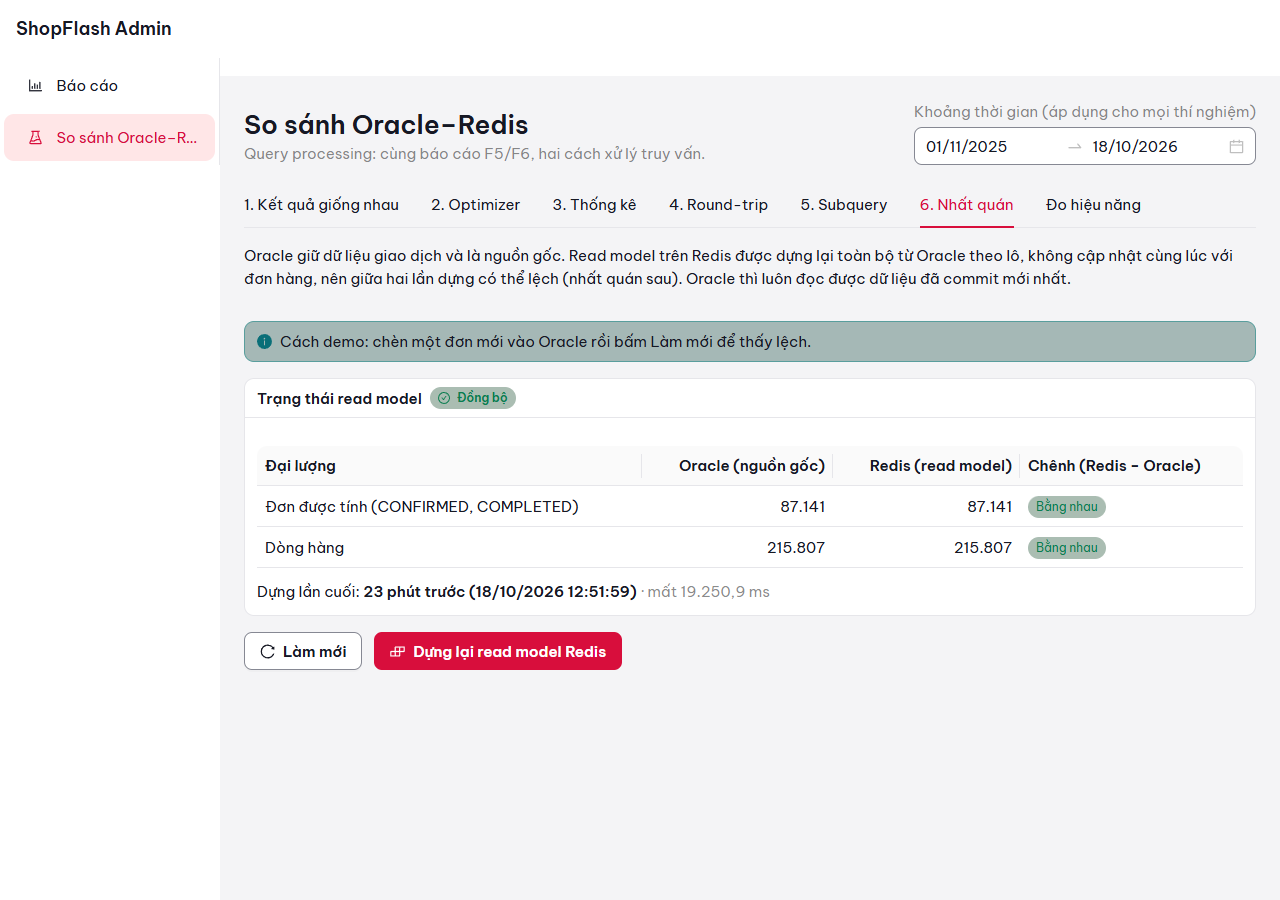
\includegraphics[width=0.75\linewidth]{3.3-08-d6-nhat-quan.png}
\caption{Tab Nhất quán: số đơn và số dòng hàng ở Oracle và Redis sau lần dựng gần nhất (19,3 s)}\label{fig:q-consistency}
\end{figure}

\paragraph{Điều phát hiện khi cài đặt}
\begin{itemize}
  \item \textbf{Phải tự khai báo \texttt{SORTABLE}.} Nếu trường dùng để \texttt{GROUPBY} hoặc \texttt{REDUCE} không được khai báo \texttt{SORTABLE}, \texttt{FT.AGGREGATE} phải đọc lại JSON của từng document. Báo cáo theo danh mục khi đó mất khoảng 1,5 s, khai báo xong còn 0,15--0,33 s (đo phía server bằng \texttt{INFO commandstats}). Bên Oracle, CBO tự chọn cách truy cập; bên Redis, lựa chọn này là việc thiết kế của lập trình viên.
  \item \textbf{Phải kèm \texttt{TIMEOUT 0}.} Redis Stack mặc định \texttt{TIMEOUT 500} với \texttt{ON\_TIMEOUT return}: lệnh quá 500 ms sẽ trả \textbf{kết quả thiếu mà không báo lỗi}. Trong lúc thử nghiệm, có lần số đơn theo trạng thái chỉ ra 2.299 vì lý do này.
  \item \textbf{Redis chạy từng lệnh một.} Trang Báo cáo gọi 5 báo cáo cùng lúc thì các lệnh \texttt{FT.AGGREGATE} phải xếp hàng chờ nhau, mỗi báo cáo hiện thời gian vài chục giây (Hình~\ref{fig:q-reports-redis}). Vì vậy số liệu so sánh chỉ lấy từ các lần đo chạy lần lượt.
  \item \textbf{Giới hạn số.} \texttt{SUM} và \texttt{AVG} của RediSearch in ra 12 chữ số có nghĩa. Dữ liệu hiện tại là VND tròn và mỗi tổng nhỏ hơn $10^{12}$ nên vẫn khớp Oracle, nhưng tổng lớn hơn sẽ mất độ chính xác.
\end{itemize}

\begin{figure}[H]
\centering
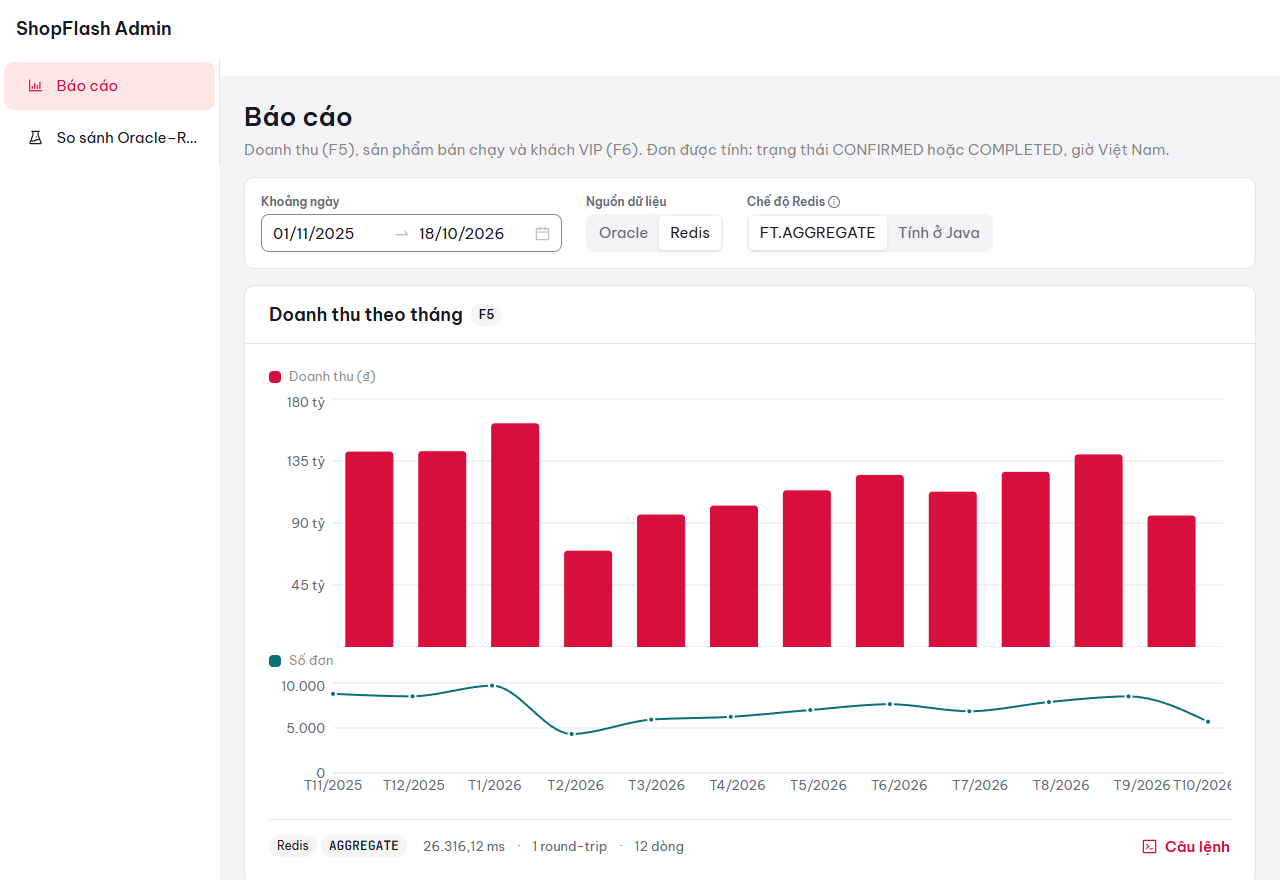
\includegraphics[width=0.75\linewidth]{3.3-02a-bao-cao-redis-dau-trang.png}
\caption{Trang Báo cáo với nguồn Redis: 5 báo cáo gửi cùng lúc nên lệnh xếp hàng, doanh thu theo tháng hiện 26.316 ms (so với 199,9 ms khi chạy riêng)}\label{fig:q-reports-redis}
\end{figure}

% ---------------------------------------------------------------------------------------------
\subsubsection{So sánh}\label{sec:q-compare}

\begin{table}[H]
\centering
\caption{Thời gian các báo cáo (ms), trung bình $\pm$ độ lệch chuẩn của 5 lần đo; p50, p95 ở \texttt{results/benchmark-summary.md}}\label{tab:q-bench}
\small\setlength{\tabcolsep}{4pt}
\begin{tabular}{@{}lrrrr@{}}
\toprule
Báo cáo & Oracle AUTO & Oracle NL (ép) & Redis AGGREGATE & Redis CLIENT \\
\midrule
Doanh thu theo tháng & \textbf{78,6 $\pm$ 17,4} & -- & 199,9 $\pm$ 22,1 & 820,1 $\pm$ 55,2 \\
Doanh thu theo danh mục & \textbf{208,5 $\pm$ 40,7} & 1.180,9 $\pm$ 227,9 & 373,4 $\pm$ 48,5 & 2.597,1 $\pm$ 382,3 \\
Top sản phẩm & \textbf{155,2 $\pm$ 23,6} & 852,9 $\pm$ 117,1 & 850,7 $\pm$ 32,4 & 4.851,2 $\pm$ 1.463,0 \\
Khách VIP & \textbf{193,7 $\pm$ 24,4} & 271,7 $\pm$ 16,9 & 875,4 $\pm$ 76,8 & 2.362,9 $\pm$ 517,2 \\
Sản phẩm chưa từng bán & \textbf{139,3 $\pm$ 22,8} & -- & không hỗ trợ & không hỗ trợ \\
\bottomrule
\end{tabular}
\end{table}

\begin{figure}[H]
\centering
\begin{tikzpicture}
\begin{axis}[
  ybar, bar width=7pt, width=0.95\linewidth, height=7cm,
  ymode=log, log origin=infty, ymin=50, ymax=8000,
  ytick={50,100,200,500,1000,2000,5000}, log ticks with fixed point,
  yticklabel style={/pgf/number format/.cd, use comma, 1000 sep={.}},
  ylabel={Thời gian (ms, thang log)},
  symbolic x coords={thang,danhmuc,top,vip},
  xticklabels={Doanh thu theo tháng, Doanh thu theo danh mục, Top sản phẩm, Khách VIP},
  xtick=data, x tick label style={font=\small, text width=2.6cm, align=center},
  legend style={at={(0.5,1.02)}, anchor=south, legend columns=4, font=\small, draw=none},
  error bars/y dir=both, error bars/y explicit,
  ymajorgrids, grid style={gray!25}, enlarge x limits=0.15,
]
\addplot+[fill=red!70!black, draw=red!70!black, error bars/error bar style={black}]
  coordinates {(thang,78.6) +- (0,17.4) (danhmuc,208.5) +- (0,40.7) (top,155.2) +- (0,23.6) (vip,193.7) +- (0,24.4)};
\addplot+[fill=red!25, draw=red!70!black, error bars/error bar style={black}]
  coordinates {(danhmuc,1180.9) +- (0,227.9) (top,852.9) +- (0,117.1) (vip,271.7) +- (0,16.9)};
\addplot+[fill=teal!80!black, draw=teal!80!black, error bars/error bar style={black}]
  coordinates {(thang,199.9) +- (0,22.1) (danhmuc,373.4) +- (0,48.5) (top,850.7) +- (0,32.4) (vip,875.4) +- (0,76.8)};
\addplot+[fill=teal!25, draw=teal!80!black, error bars/error bar style={black}]
  coordinates {(thang,820.1) +- (0,55.2) (danhmuc,2597.1) +- (0,382.3) (top,4851.2) +- (0,1463.0) (vip,2362.9) +- (0,517.2)};
\legend{Oracle AUTO, Oracle NL (ép), Redis AGGREGATE, Redis CLIENT}
\end{axis}
\end{tikzpicture}
\caption{Thời gian các báo cáo trên hai DBMS (vẽ từ Bảng~\ref{tab:q-bench}; thanh lỗi: $\pm$ 1 độ lệch chuẩn)}\label{fig:q-bench}
\end{figure}

\begin{table}[H]
\centering
\caption{So sánh xử lý truy vấn trên Oracle và Redis}\label{tab:q-criteria}
\small
\begin{tabularx}{\linewidth}{@{}>{\raggedright\arraybackslash}p{2.6cm}XX>{\raggedright\arraybackslash}p{1.8cm}@{}}
\toprule
Tiêu chí & Oracle & Redis (RediSearch) & Bằng chứng \\
\midrule
Ngôn ngữ truy vấn & SQL khai báo: join, subquery, \texttt{NOT EXISTS}, Top-N & Pipeline \texttt{FT.AGGREGATE} theo thứ tự cố định, không join, không subquery & Demo 4, 6, 8 \\
Bộ tối ưu & CBO chọn thuật toán join, cách truy cập, tự viết lại truy vấn (group-by placement, anti-join) & Không có. Lệnh viết thế nào chạy thế ấy & Demo 1, 6 \\
Kế hoạch tự chọn so với cách tệ & AUTO nhanh hơn NL ép 5,5--5,7 lần & Lập trình viên tự chọn: AGGREGATE nhanh hơn CLIENT 2,7--7 lần & Demo 2, 7 \\
Phụ thuộc thống kê & Mất thống kê: ước lượng 285K thay vì 9K dòng, đổi kế hoạch, đọc gấp 17,8 lần block & Không dùng thống kê. Hiệu năng phụ thuộc thiết kế index (\texttt{SORTABLE}) & Demo 3; điều phát hiện \\
Xem kế hoạch & \texttt{DBMS\_XPLAN.DISPLAY\_CURSOR}: E-Rows, A-Rows, Buffers từng bước & \texttt{FT.PROFILE}: số document qua từng bước & Demo 1, 6 \\
Join & Lúc truy vấn, 3 thuật toán & Không có. Join sẵn lúc dựng read model (denormalize) & Demo 1, 6 \\
Thời gian báo cáo (100k đơn) & 79--209 ms & 200--875 ms (AGGREGATE) & Bảng~\ref{tab:q-bench} \\
Subquery & 1 câu, subquery không phụ thuộc chỉ tính 1 lần & VIP: 2 lượt, ứng dụng chuyển giá trị giữa hai lượt. \texttt{NOT EXISTS}: không làm được & Demo 4, 8 \\
Độ mới của dữ liệu & Luôn đọc dữ liệu đã commit mới nhất & Chỉ đúng tới lần dựng read model gần nhất (dựng lại mất 20--35 s) & Demo 9 \\
Câu hỏi mới chưa tính trước & Viết thêm câu SQL là chạy & Có thể phải đổi read model, index và dựng lại & Demo 8 \\
\bottomrule
\end{tabularx}
\end{table}

\textbf{Nhận xét chung:}
\begin{itemize}
  \item Với truy vấn phân tích (lọc gần hết dữ liệu, join nhiều bảng, gom nhóm, subquery), Oracle nhanh hơn Redis ở mọi báo cáo đo được, từ 1,8 đến 5,5 lần, dù Oracle Free bị giới hạn 2 CPU và 2 GB RAM.
  \item Lý do không nằm ở việc đĩa hay RAM. Oracle có bộ tối ưu dựa trên thống kê, có hash join và gom nhóm bằng bảng băm phù hợp với khối dữ liệu lớn, và tự viết lại truy vấn. Redis xử lý từng lệnh trên một luồng và chỉ có một pipeline cố định.
  \item Redis mạnh ở truy cập theo key và truy vấn ngắn, không phải ở quét và gom hàng trăm nghìn document.
  \item Hai điểm khác biệt quan trọng nhất về cách xử lý truy vấn:
  \begin{enumerate}
    \item Ở Oracle, \textbf{DBMS} quyết định cách chạy. Ở Redis, \textbf{lập trình viên} quyết định, qua cách thiết kế read model, index và lệnh.
    \item Oracle chạy được những câu hỏi chưa tính trước. Redis chỉ trả lời tốt những câu hỏi đã được chuẩn bị dữ liệu sẵn.
  \end{enumerate}
\end{itemize}

% ---------------------------------------------------------------------------------------------
\subsubsection{Kết luận cho ShopFlash}\label{sec:q-conclusion}

Báo cáo doanh thu (F5) và top sản phẩm, khách VIP, sản phẩm chưa bán (F6) là truy vấn phân tích trên dữ liệu đơn hàng: cần join nhiều bảng, gom nhóm, subquery, và cần số liệu đúng tới đơn vừa đặt. ShopFlash chạy các báo cáo này trên \textbf{Oracle}:
\begin{itemize}
  \item Trang Tổng quan quản trị và trang Báo cáo mặc định đọc từ Oracle.
  \item Oracle nhanh hơn ở mọi báo cáo đo được.
  \item Oracle làm được cả báo cáo cần anti-join.
  \item Oracle không cần một bản sao dữ liệu phải dựng lại.
  \item Khi nhóm thêm báo cáo mới, chỉ cần viết thêm câu SQL.
\end{itemize}

Read model analytics trên Redis vẫn được giữ trong ứng dụng để phục vụ trang So sánh Oracle--Redis. Nó minh họa cái giá của cách làm ``tính sẵn cho câu hỏi đã biết'': phải denormalize, phải tự thiết kế index \texttt{SORTABLE}, phải dựng lại khi dữ liệu đổi. Nếu sau này có một chỉ số cần đọc rất nhiều lần với độ trễ thấp (ví dụ doanh thu đang chạy trong flash sale), cách hợp lý trên Redis là cộng dồn sẵn vào một key mỗi khi có đơn, đọc theo key, chứ không phải chạy \texttt{FT.AGGREGATE} trên toàn bộ đơn hàng.


\bibliographystyle{IEEEtran}
\bibliography{query}

\end{document}
